\section{Annisa Fathoroni/1164067}
\subsection{Teori}
\subsubsection{Soal No. 1}
Kenapa file teks harus dilakukan tokenizer, dilengkapi dengan ilustrasi atau gambar.

Karena tokenizer ini berfungsi untuk mengkonversi teks menjadi urutan integer indeks kata atau vektor binary, word count atau tf-idf. Text harus dilakukan tokenizer agar dapat dirubah menjadi vektor. Dari perubahan ke vektor tersebut maka data/textnya dapat dibaca oleh komputer (terkomputerisasi).

\begin{itemize}
\item Ilustrasi Gambar:

\begin{figure}[!hbtp]
\centering
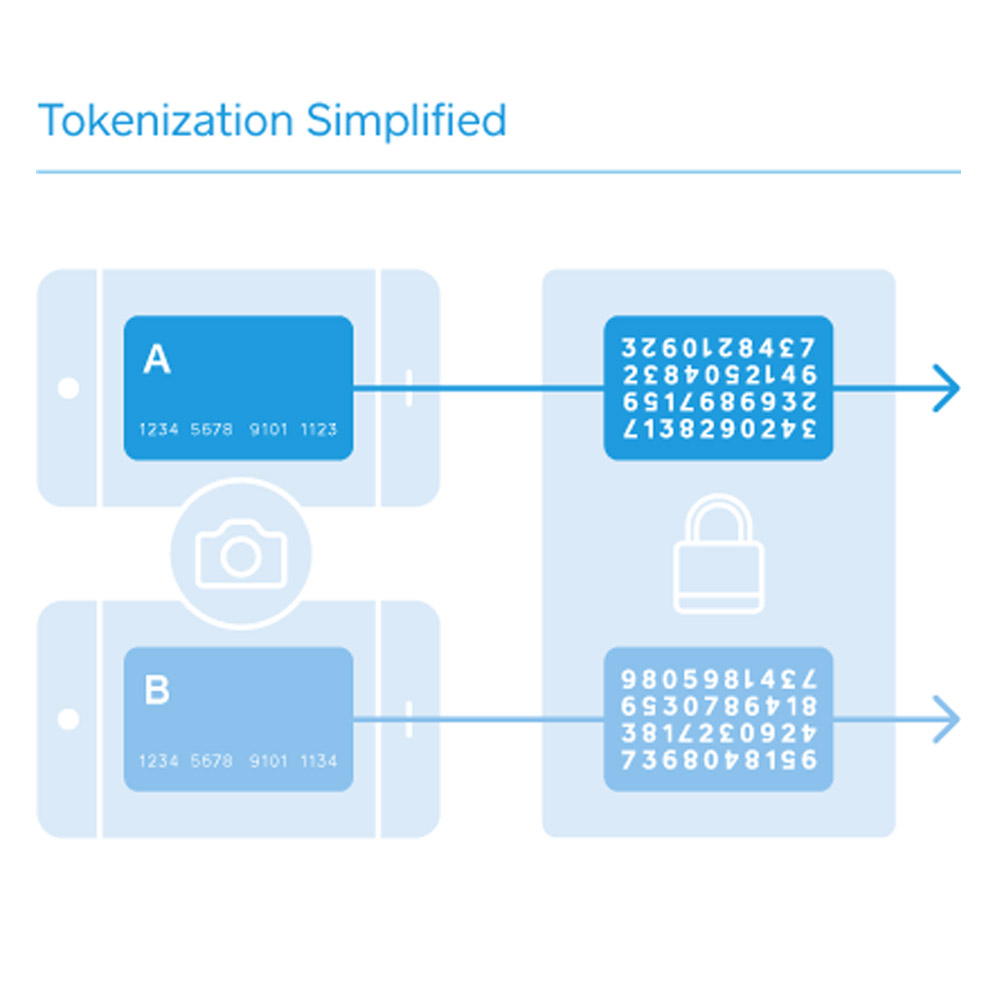
\includegraphics[scale=0.2]{figures/Chapter 7/1164067/Teori/Chapter7AnnisaFathoroni1.jpg}
\caption{Tokenizer - Annisa Fathoroni}
\label{Tokenizer - Annisa Fathoroni}
\end{figure}

\end{itemize}

\subsubsection{Soal No. 2}
Konsep dasar K Fold Cross Validation pada dataset komentar Youtube, dilengkapi dengan ilustrasi atau gambar.

Pada StartiedKFold memiliki input untuk setiap class yang terbagi menjadi 5 class pada setiap class-nya. Lalu dimasukkan kedalam class dataset youtube.

\begin{itemize}
\item Ilustrasi Gambar:

\begin{figure}[!hbtp]
\centering
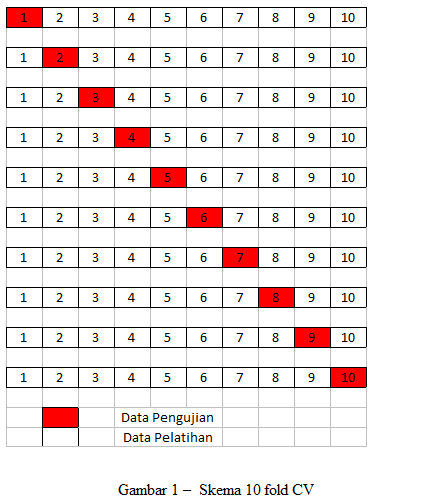
\includegraphics[scale=0.5]{figures/Chapter 7/1164067/Teori/Chapter7AnnisaFathoroni2.png}
\caption{Konsep dasar K Fold Cross Validation - Annisa Fathoroni}
\label{Konsep dasar K Fold Cross Validation - Annisa Fathoroni}
\end{figure}

\end{itemize}

\subsubsection{Soal No. 3}
Maksud kode program for train dan test in splits, dilengkapi dengan ilustrasi atau gambar.

Untuk melakukan pengujian atas data pada dataset sudah di tidak terjadi penumpukan dan split. Dimana di setiap class tidak akan muncul id yang sama.

\begin{itemize}
\item Ilustrasi Gambar :

\begin{figure}[!hbtp]
\centering
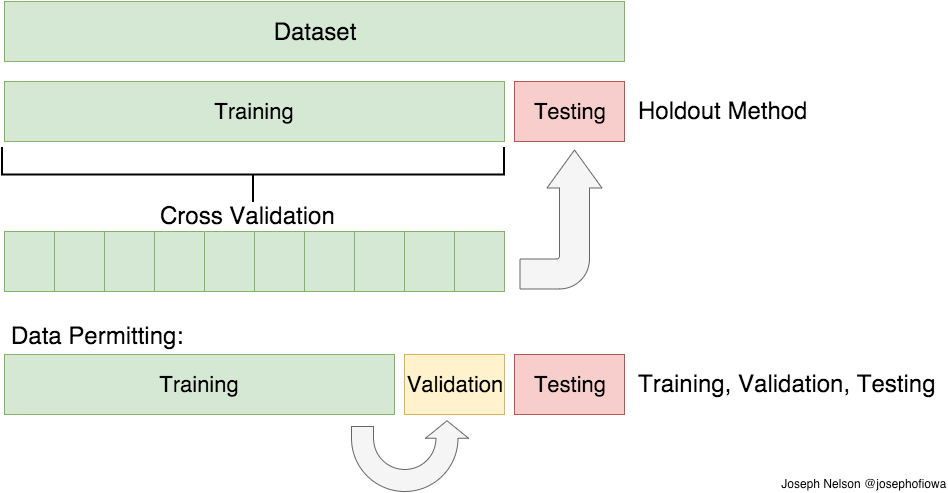
\includegraphics[scale=0.2]{figures/Chapter 7/1164067/Teori/Chapter7AnnisaFathoroni3.png}
\caption{Train dan Test in Split- Annisa Fathoroni}
\label{Train dan Test in Split- Annisa Fathoroni}
\end{figure}

\end{itemize}

\subsubsection{Soal No. 4}
Maksud kode program train content = d[’CONTENT’].iloc[train idx] dan test content = d[’CONTENT’].iloc[test idx], dilengkapi dengan ilustrasi atau gambar.

Untuk mengambil data pada kolom  CONTENT yang merupakan bagian dari train idx dan test idx.

\begin{itemize}
\item Ilustrasi Gambar:

\begin{figure}[!hbtp]
\centering
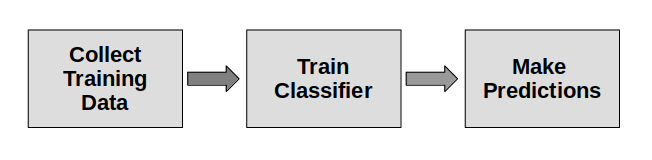
\includegraphics[scale=0.4]{figures/Chapter 7/1164067/Teori/Chapter7AnnisaFathoroni4.png}
\caption{Train content - Annisa Fathoroni}
\label{Train content - Annisa Fathoroni}
\end{figure}

\end{itemize}

\subsubsection{Soal No. 5}
Maksud dari fungsi tokenizer = Tokenizer(num words=2000) dan tokenizer.fit on texts(train content), dilengkapi dengan ilustrasi atau gambar.

Yang pertama, yaitu fungsi tokenizer ialah mem-vektorisasi jumlah kata yang ingin diubah kedalam bentuk token 2000 kata.

Yang kedua, untuk melakukan fit tokenizer untuk dat trainnya dengan data test nya untuk kolom CONTENT saja.

\begin{itemize}
\item Ilustrasi Gambar :

\begin{figure}[!hbtp]
\centering
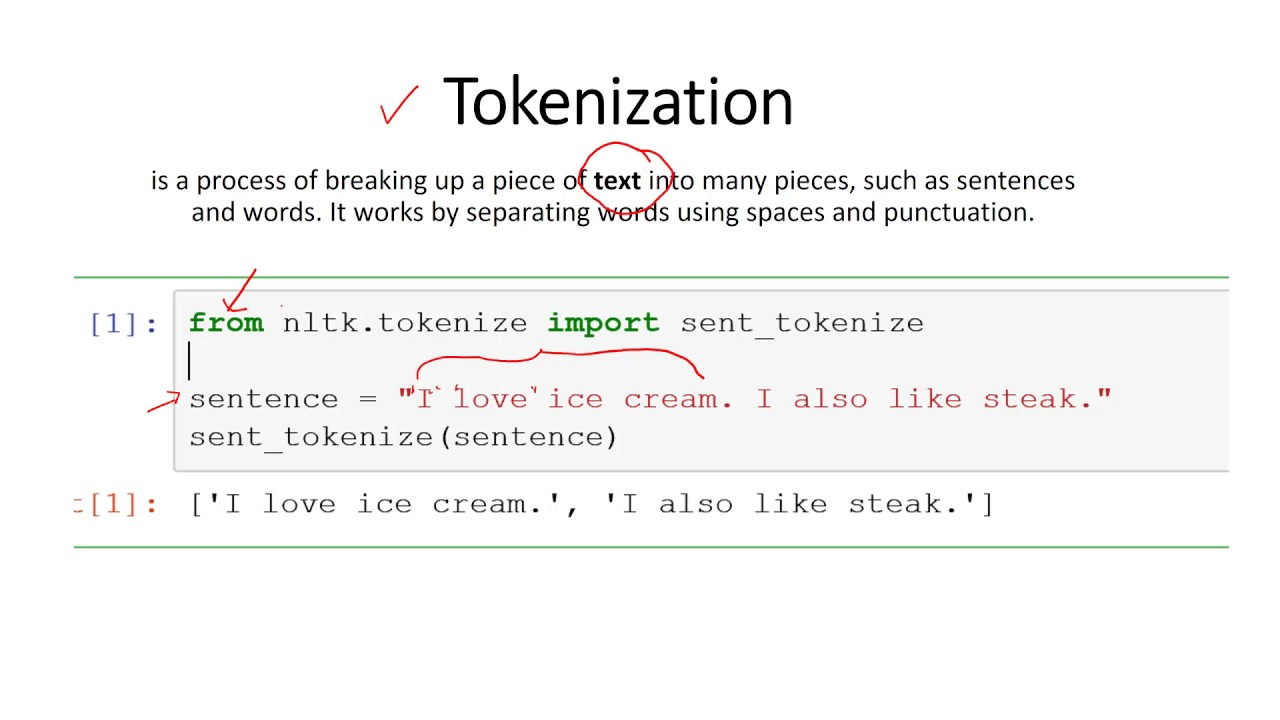
\includegraphics[scale=0.2]{figures/Chapter 7/1164067/Teori/Chapter7AnnisaFathoroni5.png}
\caption{Tokenizer - Annisa Fathoroni}
\label{Tokenizer - Annisa Fathoroni}
\end{figure}

\end{itemize}

\subsubsection{Soal No. 6}
Maksud dari fungsi d train inputs = tokenizer.texts to matrix(train content, mode=’tfidf ’) dan d test inputs = tokenizer.texts to matrix(test content, mode=’tfidf ’), dilengkapi dengan ilustrasi atau gambar.

Variabel d train input untukmelakukan tokenizer dari bentuk teks ke matrix dari data train content dengan mode tfidf dan variabel d test inputs sama saja untuk data test.

\begin{itemize}
\item Ilustrasi Gambar:

\begin{figure}[!hbtp]
\centering
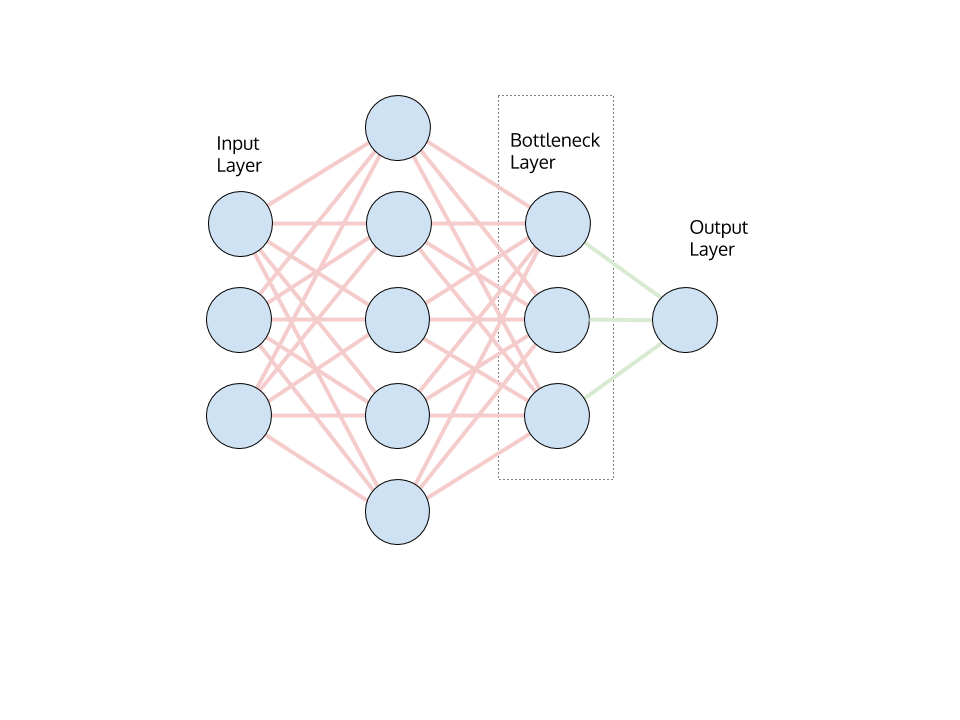
\includegraphics[scale=0.3]{figures/Chapter 7/1164067/Teori/Chapter7AnnisaFathoroni6.png}
\caption{Train Inputs 1 - Annisa Fathoroni}
\label{Train Inputs 1 - Annisa Fathoroni}
\end{figure}

\end{itemize}

\subsubsection{Soal No. 7}
Maksud dari fungsi d train inputs = d train inputs/np.amax(np.absolute(d train inputs) dan d test inputs = d test inputs/np.amax(np.absolute(d test inputs) , dilengkapi dengan ilustrasi atau gambar.

Akan membagi matrix tfidf dengan amax untuk mengembalikan array atau maksimum array. Kemudian hasilnya dimasukan dalam variabel d train inputs untuk data train dan d test inputs untuk data test dengan nominal bilangan tanpa ada bilangan negatif dan koma.

\begin{itemize}
\item Ilustrasi Gambar :

\begin{figure}[!hbtp]
\centering
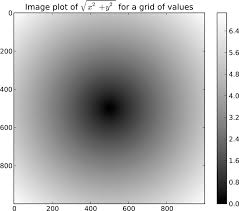
\includegraphics[scale=0.4]{figures/Chapter 7/1164067/Teori/Chapter7AnnisaFathoroni7.png}
\caption{Train Inputs 2 - Annisa Fathoroni}
\label{Train Inputs 2 - Annisa Fathoroni}
\end{figure}

\end{itemize}

\subsubsection{Soal No. 8}
 Maksud dari  d train outputs = np utils.to categorical(d[’CLASS’].iloc[train idx]) dan d test outputs = np utils.to categorical(d[’CLASS’].iloc[test idx])

Fungsi pada kode program tersebut ditujukan untuk melakukan one-hot encoding supaya bisa masuk dan digunakan pada neural network. One-hot encoding diambil dari class yang berarti hanya terdapat 2 neuron, yaitu satu nol(1,0) atau nol satu(0,1) karena pilihannya hanya ada dua.

\begin{itemize}
\item Ilustrasi Gambar:

\begin{figure}[!hbtp]
\centering
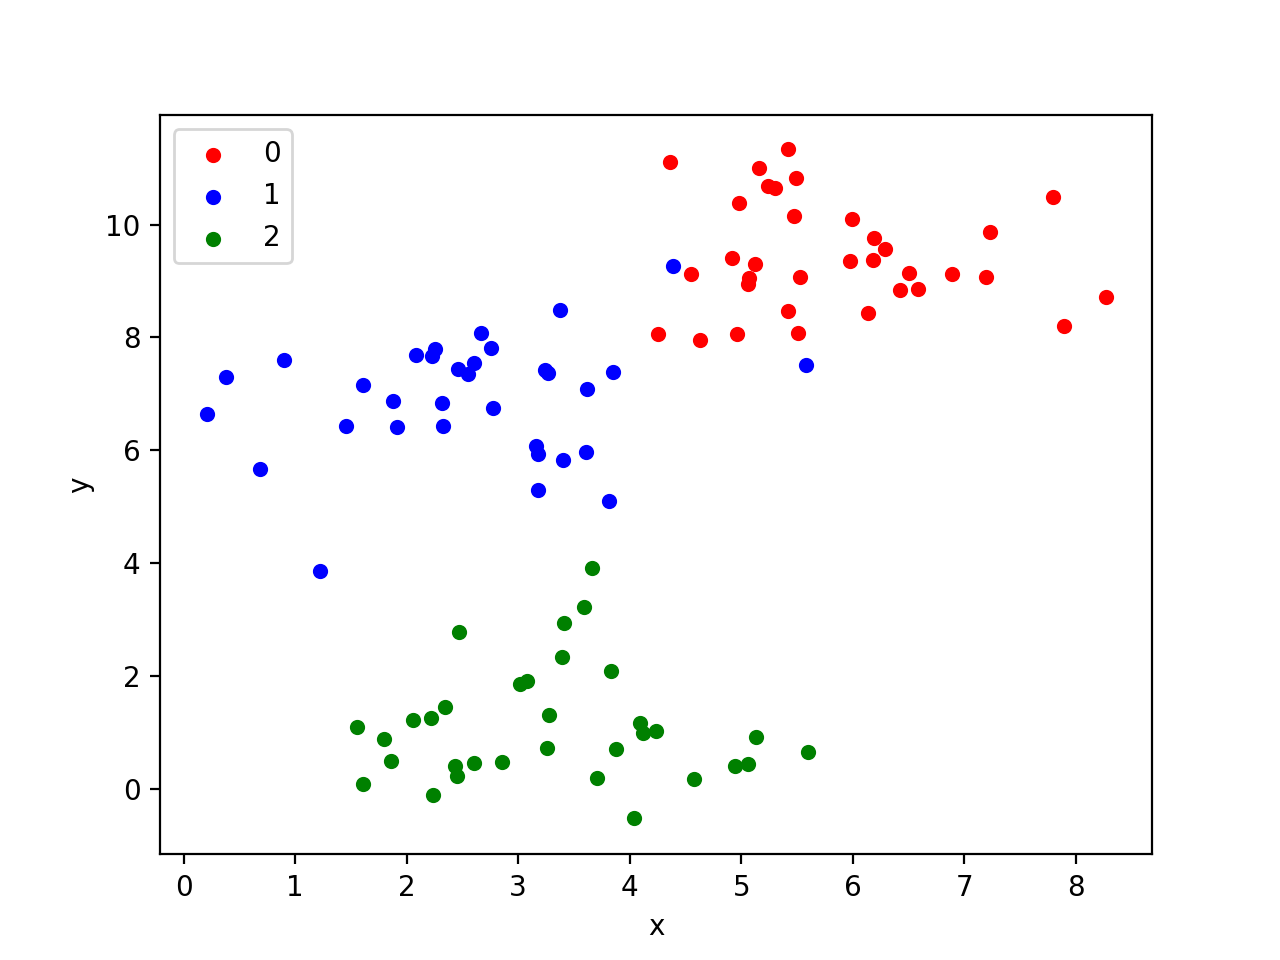
\includegraphics[scale=0.4]{figures/Chapter 7/1164067/Teori/Chapter7AnnisaFathoroni8.png}
\caption{Compile model - Annisa Fathoroni}
\label{Compile model - Annisa Fathoroni}
\end{figure}

\end{itemize}

\subsubsection{Soal No. 9}
Maksud dari listing 7.2.

\hfill \break

Fungsi kode program tersebut untuk melakukan pemodelan dengan sequential, membandingkan setiap satu larik elemen dengan cara satu persatu secara beruntun.Terdapat 512 neuron inputan dengan input shape 2000 vektor yang sudah dinormalisasi. Lalu model dilakukan aktivasi dengan fungsi 'relu'. Kemudian pemotongan bobot supaya tidak overfitting sebesar 50 persen dari neuron inputan 512. Lalu pada layer output terdapat 2 neuron outputan yaitu nol (1,0) atau nol satu (0,1). Kemudian outputan tersebut diaktivasi menggunakan fungsi softmax.

\subsubsection{Soal No. 10}
Maksud dari listing 7.3.

\hfill \break

Fungsi kode program tersebut untuk model yang telah dibuat selanjutnya dicompile dengan menggunakan algoritma optimisasi, fungsi loss, dan fungsi metrik.

\subsubsection{Soal No. 11}
Deep Learning

\hfill \break

Deep learning, yang bisa diartikan sebagai rangkaian metode untuk melatih jaringan saraf buatan multi-lapisan. Ternyata, metode ini efektif dalam mengidentifikasi pola dari data. Manakala media membicarakan jaringan saraf, kemungkinan yang dimaksud adalah deep learning.

\subsubsection{Soal No. 12}
Deep Neural Network, dan apa bedanya dengan Deep Learning

\hfill \break

Algoritma DNN (Deep Neural Networks) adalah salah satu algoritma berbasis jaringan saraf yang dapat digunakan untuk pengambilan keputusan. Contoh yang dibahas kali ini adalah mengenai penentuan penerimaan pengajuan kredit sepeda motor baru berdasarkan kelompok data yang sudah ada. 

Pebedaannya dengan Deep Learning adalah terletak pada kedalaman model, deep learning adalah frasa yang digunakan untuk jaringan saraf yang kompleks.

\subsubsection{Soal No. 13}
Jelaskan dengan ilustrasi gambar buatan sendiri, bagaimana perhitungan algoritma konvolusi dengan ukuran stride (NPM mod3+1)x(NPM mod3+1) yang terdapat max pooling.(nilai 30)

Karena NPM saya 1164067 dan hasil dari (NPM mod 3)+1 = 2, maka saya menggunaan matrik kernel berukuran 2x2. Misalkan f(x,y) yang digunakan berukuran 3x3 dan kernel atau mask berukuran 2x2 adalah sebagai berikut:

Gambar Matriks:

\begin{figure}[!hbtp]
\centering
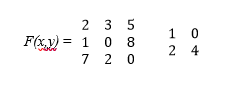
\includegraphics[scale=0.8]{figures/Chapter 7/1164067/Teori/Chapter7AnnisaFathoroni9.png}
\caption{Perhitungan algoritma konvolusi - Annisa Fathoroni}
\label{Perhitungan algoritma konvolusi - Annisa Fathoroni}
\end{figure}

Penyelesaian dari operasi konvolusi antara f(x,y) dengan kernel g(x,y)  adalah f(x,y) *  g(x,y) 

\begin{itemize}
\item  Tempatkan matrik kernel di sebelah kiri atas, lalu hitung nilai piksel pada posisi (0,0) dari kernel tersebut. Konvolusi dihitung dengan cara berikut :

(2x1) + (3x0) + (1x2) + (0x4)

Sehingga didapat hasil konvolusi = 4

\item Tempatkan matrik kernel di sebelah kanan atas, lalu hitung nilai piksel pada posisi (0,0) dari kernel tersebut. Konvolusi dihitung dengan cara berikut :

(3x1) + (5x0) + (0x2) + (8x4)

Sehingga didapat hasil konvolusi = 35

\item Tempatkan matrik kernel di sebelah kiri bawah, lalu hitung nilai piksel pada posisi (0,0) dari kernel tersebut. Konvolusi dihitung dengan cara berikut :

(1x1) + (0x0) + (7x2) + (2x4)

Sehingga didapat hasil konvolusi = 23

\item Tempatkan matrik kernel di sebelah kanan bawah, lalu hitung nilai piksel pada posisi (0,0) dari kernel tersebut. Konvolusi dihitung dengan cara berikut :

(0x1) + (8x0) + (2x2) + (0x4)

Sehingga didapat hasil konvolusi = 4

Hasil:

\begin{figure}[!hbtp]
\centering
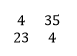
\includegraphics[scale=0.8]{figures/Chapter 7/1164067/Teori/Chapter7AnnisaFathoroni10.png}
\caption{Hasil - Annisa Fathoroni}
\label{Hasil - Annisa Fathoroni}
\end{figure}

\end{itemize}

\subsection{Praktek}


\subsection{Penanganan Error}
